% Created by tikzDevice version 0.10.1 on 2016-05-09 15:28:50
% !TEX encoding = UTF-8 Unicode
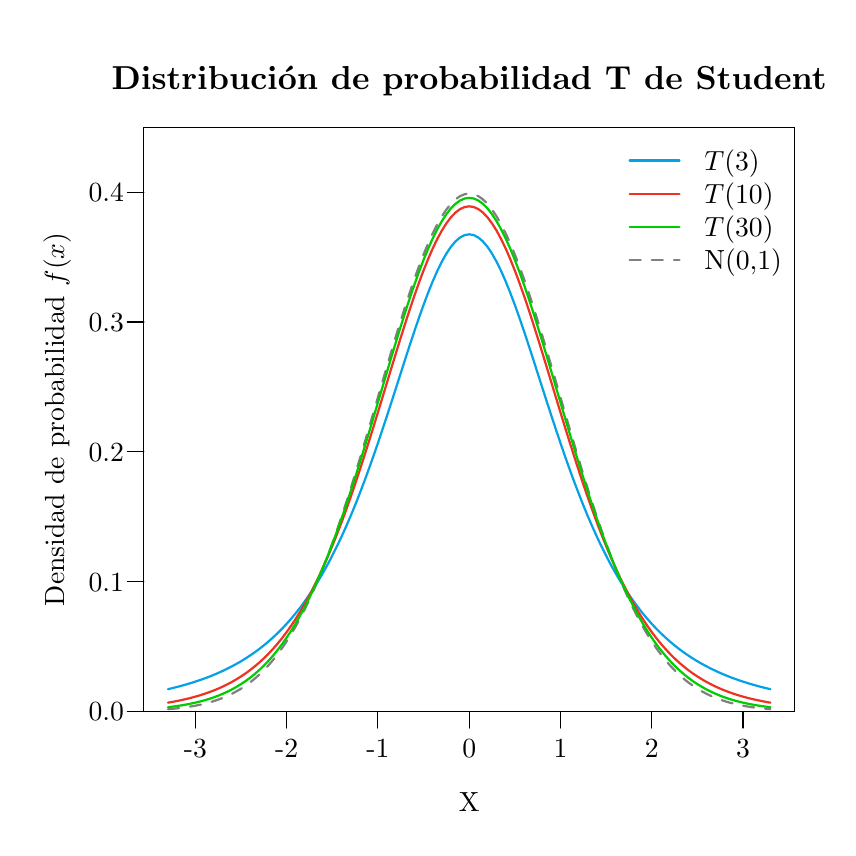
\begin{tikzpicture}[x=1pt,y=1pt]
\definecolor{fillColor}{RGB}{255,255,255}
\path[use as bounding box,fill=fillColor,fill opacity=0.00] (0,0) rectangle (289.08,289.08);
\begin{scope}
\path[clip] ( 42.00, 42.00) rectangle (277.08,253.08);
\definecolor{drawColor}{RGB}{128,128,128}

\path[draw=drawColor,line width= 0.8pt,dash pattern=on 4pt off 4pt ,line join=round,line cap=round] ( 50.71, 42.81) --
	( 52.36, 42.95) --
	( 54.00, 43.12) --
	( 55.65, 43.31) --
	( 57.30, 43.53) --
	( 58.95, 43.79) --
	( 60.60, 44.08) --
	( 62.25, 44.41) --
	( 63.90, 44.79) --
	( 65.55, 45.22) --
	( 67.20, 45.71) --
	( 68.85, 46.27) --
	( 70.49, 46.89) --
	( 72.14, 47.59) --
	( 73.79, 48.37) --
	( 75.44, 49.25) --
	( 77.09, 50.22) --
	( 78.74, 51.31) --
	( 80.39, 52.50) --
	( 82.04, 53.83) --
	( 83.69, 55.29) --
	( 85.34, 56.89) --
	( 86.98, 58.64) --
	( 88.63, 60.55) --
	( 90.28, 62.63) --
	( 91.93, 64.89) --
	( 93.58, 67.33) --
	( 95.23, 69.95) --
	( 96.88, 72.78) --
	( 98.53, 75.80) --
	(100.18, 79.03) --
	(101.83, 82.47) --
	(103.47, 86.12) --
	(105.12, 89.97) --
	(106.77, 94.03) --
	(108.42, 98.29) --
	(110.07,102.75) --
	(111.72,107.40) --
	(113.37,112.23) --
	(115.02,117.23) --
	(116.67,122.38) --
	(118.32,127.67) --
	(119.96,133.09) --
	(121.61,138.60) --
	(123.26,144.19) --
	(124.91,149.83) --
	(126.56,155.50) --
	(128.21,161.17) --
	(129.86,166.81) --
	(131.51,172.39) --
	(133.16,177.88) --
	(134.81,183.25) --
	(136.45,188.47) --
	(138.10,193.50) --
	(139.75,198.30) --
	(141.40,202.86) --
	(143.05,207.14) --
	(144.70,211.11) --
	(146.35,214.74) --
	(148.00,218.01) --
	(149.65,220.90) --
	(151.30,223.37) --
	(152.94,225.43) --
	(154.59,227.04) --
	(156.24,228.20) --
	(157.89,228.90) --
	(159.54,229.13) --
	(161.19,228.90) --
	(162.84,228.20) --
	(164.49,227.04) --
	(166.14,225.43) --
	(167.78,223.37) --
	(169.43,220.90) --
	(171.08,218.01) --
	(172.73,214.74) --
	(174.38,211.11) --
	(176.03,207.14) --
	(177.68,202.86) --
	(179.33,198.30) --
	(180.98,193.50) --
	(182.63,188.47) --
	(184.27,183.25) --
	(185.92,177.88) --
	(187.57,172.39) --
	(189.22,166.81) --
	(190.87,161.17) --
	(192.52,155.50) --
	(194.17,149.83) --
	(195.82,144.19) --
	(197.47,138.60) --
	(199.12,133.09) --
	(200.76,127.67) --
	(202.41,122.38) --
	(204.06,117.23) --
	(205.71,112.23) --
	(207.36,107.40) --
	(209.01,102.75) --
	(210.66, 98.29) --
	(212.31, 94.03) --
	(213.96, 89.97) --
	(215.61, 86.12) --
	(217.25, 82.47) --
	(218.90, 79.03) --
	(220.55, 75.80) --
	(222.20, 72.78) --
	(223.85, 69.95) --
	(225.50, 67.33) --
	(227.15, 64.89) --
	(228.80, 62.63) --
	(230.45, 60.55) --
	(232.10, 58.64) --
	(233.74, 56.89) --
	(235.39, 55.29) --
	(237.04, 53.83) --
	(238.69, 52.50) --
	(240.34, 51.31) --
	(241.99, 50.22) --
	(243.64, 49.25) --
	(245.29, 48.37) --
	(246.94, 47.59) --
	(248.59, 46.89) --
	(250.23, 46.27) --
	(251.88, 45.71) --
	(253.53, 45.22) --
	(255.18, 44.79) --
	(256.83, 44.41) --
	(258.48, 44.08) --
	(260.13, 43.79) --
	(261.78, 43.53) --
	(263.43, 43.31) --
	(265.08, 43.12) --
	(266.72, 42.95) --
	(268.37, 42.81);
\end{scope}
\begin{scope}
\path[clip] (  0.00,  0.00) rectangle (289.08,289.08);
\definecolor{drawColor}{RGB}{0,0,0}

\path[draw=drawColor,line width= 0.4pt,line join=round,line cap=round] ( 60.60, 42.00) -- (258.48, 42.00);

\path[draw=drawColor,line width= 0.4pt,line join=round,line cap=round] ( 60.60, 42.00) -- ( 60.60, 36.00);

\path[draw=drawColor,line width= 0.4pt,line join=round,line cap=round] ( 93.58, 42.00) -- ( 93.58, 36.00);

\path[draw=drawColor,line width= 0.4pt,line join=round,line cap=round] (126.56, 42.00) -- (126.56, 36.00);

\path[draw=drawColor,line width= 0.4pt,line join=round,line cap=round] (159.54, 42.00) -- (159.54, 36.00);

\path[draw=drawColor,line width= 0.4pt,line join=round,line cap=round] (192.52, 42.00) -- (192.52, 36.00);

\path[draw=drawColor,line width= 0.4pt,line join=round,line cap=round] (225.50, 42.00) -- (225.50, 36.00);

\path[draw=drawColor,line width= 0.4pt,line join=round,line cap=round] (258.48, 42.00) -- (258.48, 36.00);

\node[text=drawColor,anchor=base,inner sep=0pt, outer sep=0pt, scale=  1.00] at ( 60.60, 25.20) {-3};

\node[text=drawColor,anchor=base,inner sep=0pt, outer sep=0pt, scale=  1.00] at ( 93.58, 25.20) {-2};

\node[text=drawColor,anchor=base,inner sep=0pt, outer sep=0pt, scale=  1.00] at (126.56, 25.20) {-1};

\node[text=drawColor,anchor=base,inner sep=0pt, outer sep=0pt, scale=  1.00] at (159.54, 25.20) {0};

\node[text=drawColor,anchor=base,inner sep=0pt, outer sep=0pt, scale=  1.00] at (192.52, 25.20) {1};

\node[text=drawColor,anchor=base,inner sep=0pt, outer sep=0pt, scale=  1.00] at (225.50, 25.20) {2};

\node[text=drawColor,anchor=base,inner sep=0pt, outer sep=0pt, scale=  1.00] at (258.48, 25.20) {3};

\path[draw=drawColor,line width= 0.4pt,line join=round,line cap=round] ( 42.00, 42.00) -- ( 42.00,229.63);

\path[draw=drawColor,line width= 0.4pt,line join=round,line cap=round] ( 42.00, 42.00) -- ( 36.00, 42.00);

\path[draw=drawColor,line width= 0.4pt,line join=round,line cap=round] ( 42.00, 88.91) -- ( 36.00, 88.91);

\path[draw=drawColor,line width= 0.4pt,line join=round,line cap=round] ( 42.00,135.81) -- ( 36.00,135.81);

\path[draw=drawColor,line width= 0.4pt,line join=round,line cap=round] ( 42.00,182.72) -- ( 36.00,182.72);

\path[draw=drawColor,line width= 0.4pt,line join=round,line cap=round] ( 42.00,229.63) -- ( 36.00,229.63);

\node[text=drawColor,anchor=base east,inner sep=0pt, outer sep=0pt, scale=  1.00] at ( 34.80, 38.56) {0.0};

\node[text=drawColor,anchor=base east,inner sep=0pt, outer sep=0pt, scale=  1.00] at ( 34.80, 85.46) {0.1};

\node[text=drawColor,anchor=base east,inner sep=0pt, outer sep=0pt, scale=  1.00] at ( 34.80,132.37) {0.2};

\node[text=drawColor,anchor=base east,inner sep=0pt, outer sep=0pt, scale=  1.00] at ( 34.80,179.28) {0.3};

\node[text=drawColor,anchor=base east,inner sep=0pt, outer sep=0pt, scale=  1.00] at ( 34.80,226.18) {0.4};

\path[draw=drawColor,line width= 0.4pt,line join=round,line cap=round] ( 42.00, 42.00) --
	(277.08, 42.00) --
	(277.08,253.08) --
	( 42.00,253.08) --
	( 42.00, 42.00);
\end{scope}
\begin{scope}
\path[clip] (  0.00,  0.00) rectangle (289.08,289.08);
\definecolor{drawColor}{RGB}{0,0,0}

\node[text=drawColor,anchor=base,inner sep=0pt, outer sep=0pt, scale=  1.20] at (159.54,266.89) {\bfseries Distribución de probabilidad T de Student};

\node[text=drawColor,anchor=base,inner sep=0pt, outer sep=0pt, scale=  1.00] at (159.54,  6.00) {X};

\node[text=drawColor,rotate= 90.00,anchor=base,inner sep=0pt, outer sep=0pt, scale=  1.00] at ( 13.20,147.54) {Densidad de probabilidad $f(x)$};
\end{scope}
\begin{scope}
\path[clip] ( 42.00, 42.00) rectangle (277.08,253.08);
\definecolor{drawColor}{RGB}{5,161,230}

\path[draw=drawColor,line width= 0.8pt,line join=round,line cap=round] ( 50.71, 50.04) --
	( 52.36, 50.44) --
	( 54.00, 50.85) --
	( 55.65, 51.29) --
	( 57.30, 51.76) --
	( 58.95, 52.25) --
	( 60.60, 52.78) --
	( 62.25, 53.33) --
	( 63.90, 53.92) --
	( 65.55, 54.54) --
	( 67.20, 55.20) --
	( 68.85, 55.91) --
	( 70.49, 56.65) --
	( 72.14, 57.45) --
	( 73.79, 58.29) --
	( 75.44, 59.18) --
	( 77.09, 60.13) --
	( 78.74, 61.15) --
	( 80.39, 62.22) --
	( 82.04, 63.36) --
	( 83.69, 64.58) --
	( 85.34, 65.87) --
	( 86.98, 67.24) --
	( 88.63, 68.71) --
	( 90.28, 70.26) --
	( 91.93, 71.91) --
	( 93.58, 73.67) --
	( 95.23, 75.53) --
	( 96.88, 77.51) --
	( 98.53, 79.62) --
	(100.18, 81.85) --
	(101.83, 84.22) --
	(103.47, 86.73) --
	(105.12, 89.38) --
	(106.77, 92.19) --
	(108.42, 95.16) --
	(110.07, 98.30) --
	(111.72,101.60) --
	(113.37,105.07) --
	(115.02,108.72) --
	(116.67,112.54) --
	(118.32,116.54) --
	(119.96,120.71) --
	(121.61,125.05) --
	(123.26,129.55) --
	(124.91,134.19) --
	(126.56,138.98) --
	(128.21,143.89) --
	(129.86,148.89) --
	(131.51,153.98) --
	(133.16,159.11) --
	(134.81,164.26) --
	(136.45,169.39) --
	(138.10,174.47) --
	(139.75,179.44) --
	(141.40,184.27) --
	(143.05,188.90) --
	(144.70,193.29) --
	(146.35,197.39) --
	(148.00,201.14) --
	(149.65,204.51) --
	(151.30,207.44) --
	(152.94,209.90) --
	(154.59,211.85) --
	(156.24,213.26) --
	(157.89,214.12) --
	(159.54,214.41) --
	(161.19,214.12) --
	(162.84,213.26) --
	(164.49,211.85) --
	(166.14,209.90) --
	(167.78,207.44) --
	(169.43,204.51) --
	(171.08,201.14) --
	(172.73,197.39) --
	(174.38,193.29) --
	(176.03,188.90) --
	(177.68,184.27) --
	(179.33,179.44) --
	(180.98,174.47) --
	(182.63,169.39) --
	(184.27,164.26) --
	(185.92,159.11) --
	(187.57,153.98) --
	(189.22,148.89) --
	(190.87,143.89) --
	(192.52,138.98) --
	(194.17,134.19) --
	(195.82,129.55) --
	(197.47,125.05) --
	(199.12,120.71) --
	(200.76,116.54) --
	(202.41,112.54) --
	(204.06,108.72) --
	(205.71,105.07) --
	(207.36,101.60) --
	(209.01, 98.30) --
	(210.66, 95.16) --
	(212.31, 92.19) --
	(213.96, 89.38) --
	(215.61, 86.73) --
	(217.25, 84.22) --
	(218.90, 81.85) --
	(220.55, 79.62) --
	(222.20, 77.51) --
	(223.85, 75.53) --
	(225.50, 73.67) --
	(227.15, 71.91) --
	(228.80, 70.26) --
	(230.45, 68.71) --
	(232.10, 67.24) --
	(233.74, 65.87) --
	(235.39, 64.58) --
	(237.04, 63.36) --
	(238.69, 62.22) --
	(240.34, 61.15) --
	(241.99, 60.13) --
	(243.64, 59.18) --
	(245.29, 58.29) --
	(246.94, 57.45) --
	(248.59, 56.65) --
	(250.23, 55.91) --
	(251.88, 55.20) --
	(253.53, 54.54) --
	(255.18, 53.92) --
	(256.83, 53.33) --
	(258.48, 52.78) --
	(260.13, 52.25) --
	(261.78, 51.76) --
	(263.43, 51.29) --
	(265.08, 50.85) --
	(266.72, 50.44) --
	(268.37, 50.04);
\definecolor{drawColor}{RGB}{238,50,36}

\path[draw=drawColor,line width= 0.8pt,line join=round,line cap=round] ( 50.71, 45.17) --
	( 52.36, 45.46) --
	( 54.00, 45.78) --
	( 55.65, 46.12) --
	( 57.30, 46.49) --
	( 58.95, 46.90) --
	( 60.60, 47.35) --
	( 62.25, 47.83) --
	( 63.90, 48.36) --
	( 65.55, 48.94) --
	( 67.20, 49.56) --
	( 68.85, 50.24) --
	( 70.49, 50.98) --
	( 72.14, 51.79) --
	( 73.79, 52.66) --
	( 75.44, 53.61) --
	( 77.09, 54.64) --
	( 78.74, 55.75) --
	( 80.39, 56.95) --
	( 82.04, 58.26) --
	( 83.69, 59.66) --
	( 85.34, 61.18) --
	( 86.98, 62.82) --
	( 88.63, 64.58) --
	( 90.28, 66.47) --
	( 91.93, 68.50) --
	( 93.58, 70.68) --
	( 95.23, 73.01) --
	( 96.88, 75.50) --
	( 98.53, 78.16) --
	(100.18, 80.99) --
	(101.83, 83.99) --
	(103.47, 87.18) --
	(105.12, 90.55) --
	(106.77, 94.10) --
	(108.42, 97.85) --
	(110.07,101.78) --
	(111.72,105.90) --
	(113.37,110.20) --
	(115.02,114.68) --
	(116.67,119.33) --
	(118.32,124.13) --
	(119.96,129.09) --
	(121.61,134.18) --
	(123.26,139.38) --
	(124.91,144.68) --
	(126.56,150.06) --
	(128.21,155.48) --
	(129.86,160.92) --
	(131.51,166.36) --
	(133.16,171.76) --
	(134.81,177.08) --
	(136.45,182.29) --
	(138.10,187.36) --
	(139.75,192.25) --
	(141.40,196.92) --
	(143.05,201.34) --
	(144.70,205.46) --
	(146.35,209.26) --
	(148.00,212.70) --
	(149.65,215.74) --
	(151.30,218.37) --
	(152.94,220.55) --
	(154.59,222.28) --
	(156.24,223.52) --
	(157.89,224.27) --
	(159.54,224.52) --
	(161.19,224.27) --
	(162.84,223.52) --
	(164.49,222.28) --
	(166.14,220.55) --
	(167.78,218.37) --
	(169.43,215.74) --
	(171.08,212.70) --
	(172.73,209.26) --
	(174.38,205.46) --
	(176.03,201.34) --
	(177.68,196.92) --
	(179.33,192.25) --
	(180.98,187.36) --
	(182.63,182.29) --
	(184.27,177.08) --
	(185.92,171.76) --
	(187.57,166.36) --
	(189.22,160.92) --
	(190.87,155.48) --
	(192.52,150.06) --
	(194.17,144.68) --
	(195.82,139.38) --
	(197.47,134.18) --
	(199.12,129.09) --
	(200.76,124.13) --
	(202.41,119.33) --
	(204.06,114.68) --
	(205.71,110.20) --
	(207.36,105.90) --
	(209.01,101.78) --
	(210.66, 97.85) --
	(212.31, 94.10) --
	(213.96, 90.55) --
	(215.61, 87.18) --
	(217.25, 83.99) --
	(218.90, 80.99) --
	(220.55, 78.16) --
	(222.20, 75.50) --
	(223.85, 73.01) --
	(225.50, 70.68) --
	(227.15, 68.50) --
	(228.80, 66.47) --
	(230.45, 64.58) --
	(232.10, 62.82) --
	(233.74, 61.18) --
	(235.39, 59.66) --
	(237.04, 58.26) --
	(238.69, 56.95) --
	(240.34, 55.75) --
	(241.99, 54.64) --
	(243.64, 53.61) --
	(245.29, 52.66) --
	(246.94, 51.79) --
	(248.59, 50.98) --
	(250.23, 50.24) --
	(251.88, 49.56) --
	(253.53, 48.94) --
	(255.18, 48.36) --
	(256.83, 47.83) --
	(258.48, 47.35) --
	(260.13, 46.90) --
	(261.78, 46.49) --
	(263.43, 46.12) --
	(265.08, 45.78) --
	(266.72, 45.46) --
	(268.37, 45.17);
\definecolor{drawColor}{RGB}{0,205,0}

\path[draw=drawColor,line width= 0.8pt,line join=round,line cap=round] ( 50.71, 43.53) --
	( 52.36, 43.73) --
	( 54.00, 43.96) --
	( 55.65, 44.21) --
	( 57.30, 44.50) --
	( 58.95, 44.82) --
	( 60.60, 45.18) --
	( 62.25, 45.58) --
	( 63.90, 46.03) --
	( 65.55, 46.52) --
	( 67.20, 47.08) --
	( 68.85, 47.69) --
	( 70.49, 48.37) --
	( 72.14, 49.12) --
	( 73.79, 49.95) --
	( 75.44, 50.87) --
	( 77.09, 51.88) --
	( 78.74, 52.98) --
	( 80.39, 54.20) --
	( 82.04, 55.52) --
	( 83.69, 56.97) --
	( 85.34, 58.55) --
	( 86.98, 60.27) --
	( 88.63, 62.13) --
	( 90.28, 64.15) --
	( 91.93, 66.32) --
	( 93.58, 68.67) --
	( 95.23, 71.19) --
	( 96.88, 73.89) --
	( 98.53, 76.78) --
	(100.18, 79.86) --
	(101.83, 83.13) --
	(103.47, 86.61) --
	(105.12, 90.28) --
	(106.77, 94.16) --
	(108.42, 98.23) --
	(110.07,102.49) --
	(111.72,106.95) --
	(113.37,111.58) --
	(115.02,116.39) --
	(116.67,121.36) --
	(118.32,126.48) --
	(119.96,131.73) --
	(121.61,137.09) --
	(123.26,142.54) --
	(124.91,148.07) --
	(126.56,153.63) --
	(128.21,159.22) --
	(129.86,164.80) --
	(131.51,170.33) --
	(133.16,175.79) --
	(134.81,181.15) --
	(136.45,186.37) --
	(138.10,191.41) --
	(139.75,196.25) --
	(141.40,200.85) --
	(143.05,205.18) --
	(144.70,209.20) --
	(146.35,212.89) --
	(148.00,216.22) --
	(149.65,219.16) --
	(151.30,221.69) --
	(152.94,223.78) --
	(154.59,225.43) --
	(156.24,226.62) --
	(157.89,227.34) --
	(159.54,227.58) --
	(161.19,227.34) --
	(162.84,226.62) --
	(164.49,225.43) --
	(166.14,223.78) --
	(167.78,221.69) --
	(169.43,219.16) --
	(171.08,216.22) --
	(172.73,212.89) --
	(174.38,209.20) --
	(176.03,205.18) --
	(177.68,200.85) --
	(179.33,196.25) --
	(180.98,191.41) --
	(182.63,186.37) --
	(184.27,181.15) --
	(185.92,175.79) --
	(187.57,170.33) --
	(189.22,164.80) --
	(190.87,159.22) --
	(192.52,153.63) --
	(194.17,148.07) --
	(195.82,142.54) --
	(197.47,137.09) --
	(199.12,131.73) --
	(200.76,126.48) --
	(202.41,121.36) --
	(204.06,116.39) --
	(205.71,111.58) --
	(207.36,106.95) --
	(209.01,102.49) --
	(210.66, 98.23) --
	(212.31, 94.16) --
	(213.96, 90.28) --
	(215.61, 86.61) --
	(217.25, 83.13) --
	(218.90, 79.86) --
	(220.55, 76.78) --
	(222.20, 73.89) --
	(223.85, 71.19) --
	(225.50, 68.67) --
	(227.15, 66.32) --
	(228.80, 64.15) --
	(230.45, 62.13) --
	(232.10, 60.27) --
	(233.74, 58.55) --
	(235.39, 56.97) --
	(237.04, 55.52) --
	(238.69, 54.20) --
	(240.34, 52.98) --
	(241.99, 51.88) --
	(243.64, 50.87) --
	(245.29, 49.95) --
	(246.94, 49.12) --
	(248.59, 48.37) --
	(250.23, 47.69) --
	(251.88, 47.08) --
	(253.53, 46.52) --
	(255.18, 46.03) --
	(256.83, 45.58) --
	(258.48, 45.18) --
	(260.13, 44.82) --
	(261.78, 44.50) --
	(263.43, 44.21) --
	(265.08, 43.96) --
	(266.72, 43.73) --
	(268.37, 43.53);
\definecolor{drawColor}{RGB}{5,161,230}

\path[draw=drawColor,line width= 0.8pt,line join=round,line cap=round] (217.52,241.08) -- (235.52,241.08);
\definecolor{drawColor}{RGB}{238,50,36}

\path[draw=drawColor,line width= 0.8pt,line join=round,line cap=round] (217.52,229.08) -- (235.52,229.08);
\definecolor{drawColor}{RGB}{0,205,0}

\path[draw=drawColor,line width= 0.8pt,line join=round,line cap=round] (217.52,217.08) -- (235.52,217.08);
\definecolor{drawColor}{RGB}{128,128,128}

\path[draw=drawColor,line width= 0.8pt,dash pattern=on 4pt off 4pt ,line join=round,line cap=round] (217.52,205.08) -- (235.52,205.08);
\definecolor{drawColor}{RGB}{0,0,0}

\node[text=drawColor,anchor=base west,inner sep=0pt, outer sep=0pt, scale=  1.00] at (244.52,237.64) {$T(3)$};

\node[text=drawColor,anchor=base west,inner sep=0pt, outer sep=0pt, scale=  1.00] at (244.52,225.64) {$T(10)$};

\node[text=drawColor,anchor=base west,inner sep=0pt, outer sep=0pt, scale=  1.00] at (244.52,213.64) {$T(30)$};

\node[text=drawColor,anchor=base west,inner sep=0pt, outer sep=0pt, scale=  1.00] at (244.52,201.64) {N(0,1)};
\end{scope}
\begin{scope}
\path[clip] (  0.00,  0.00) rectangle (289.08,289.08);
\definecolor{drawColor}{RGB}{0,0,0}

\path[draw=drawColor,line width= 0.4pt,line join=round,line cap=round] ( 42.00, 42.00) --
	(277.08, 42.00) --
	(277.08,253.08) --
	( 42.00,253.08) --
	( 42.00, 42.00);
\end{scope}
\end{tikzpicture}
